\documentclass{article}
\usepackage[utf8]{inputenc}
\usepackage{pgfplots}
\pgfplotsset{width=10cm,compat=1.9}
\usepackage{amsmath,amssymb,amsthm}
\usepackage{graphicx}
\usepackage{float}
\usepackage{blindtext}
\usepackage{hyperref}
\usepackage{verbatim}
\usepackage{gensymb}
\usepackage{enumerate}
\usepackage{xcolor}
\usepackage{graphicx}
\hypersetup{
    colorlinks=true,
    linkcolor=blue,
    filecolor=magenta,      
    urlcolor=cyan,
    pdftitle={Overleaf Example},
    pdfpagemode=FullScreen,
    }
\usepackage[slovene]{babel}

\setlength{\parindent}{0pt}
\setlength{\parskip}{4pt}

\newcounter{example}[section]
\newenvironment{example}[1][]{\refstepcounter{example}\par\medskip
   \noindent \textbf{Naloga~\theexample. #1} \rmfamily}{\medskip}

\newtheorem*{zgled}{Zgled}

\title{Vektorji}
\author{Bor Bregant}
\date{\vspace{-5ex}}

\begin{document}

\thispagestyle{empty}	% ne oštevilči strani

\noindent MATEMATIKA, \quad 2. B \hfill Škofijska klasična gimnazija
\hrule
\vspace{1ex}
\noindent \textbf{Tema: Odvisni in neodvisni vektorji}
\vspace{1ex}

\noindent \textbf{Enota: Vektorji}
\vspace{1ex}

\noindent \textbf{Datum: 26. 10. 2023}
\vspace{1ex}

\noindent \textbf{Mentorica: dr. Marina Rugelj}
\vspace{1ex}

\noindent \textbf{Viri in literatura: Planum novum, 2020, Pavlič G. in drugi}
\vspace{1ex}
\hrule
\vspace{2ex}
\noindent \textbf{Učne oblike: Frontalna, individualna}
\vspace{1ex}

\noindent \textbf{Učne metode: Metoda razprave v uvodu, razlaga}
\vspace{1ex}

\noindent \textbf{Učni pripomočki: Tabla, učbenik}
\vspace{1ex}

\noindent \textbf{Učni cilji: Dijaki/dijakinje znajo množiti vektorje s skalarjem na grafičnem nivoju.} 
\vspace{4ex}
\hrule
\vspace{5ex}
\noindent \textbf{Vsebina in potek:} 

\newpage

\section*{\textcolor{violet}{Vžig in uvod}}

Po pozdravu pregledamo morebitna vprašanja glede domače naloge in včerajšnje snovi.

Začnemo z uvodom množenja vektorjev s številom v razpravi. Razmišljamo, kaj bi se zgodilo, če seštevamo enaka vektorja. \textcolor{violet}{Dijaki pri pogovoru sodelujejo.}


\section*{\textcolor{violet}{Razlaga snovi}}

\textbf{Odvisni in neodvisni vektorji}

Vektorja $\vec{a}$ in $\vec{b}$ sta \textbf{linearno odvisna}, če lahko enega izrazimo z drugim $\vec{a}=k\cdot \vec{b}$. Vektorja ležita na vzporednih nosilkah in rečemo, da sta kolinearna.

Dva vektorja $\vec{a}$ in $\vec{b}$ v ravnini, ki nista kolinearna sta \textbf{linearno neodvisna} in tvoria \textbf{bazo} ravnine. To pomeni, da lahko vsak vektor v ravnini na en sam način zapišemo kot njuno \textbf{linearno kombinacijo}:
\[\vec{v}=m\vec{a}+n\vec{b};\ m,n\in\mathbb{R}\]

\begin{figure}[H]
    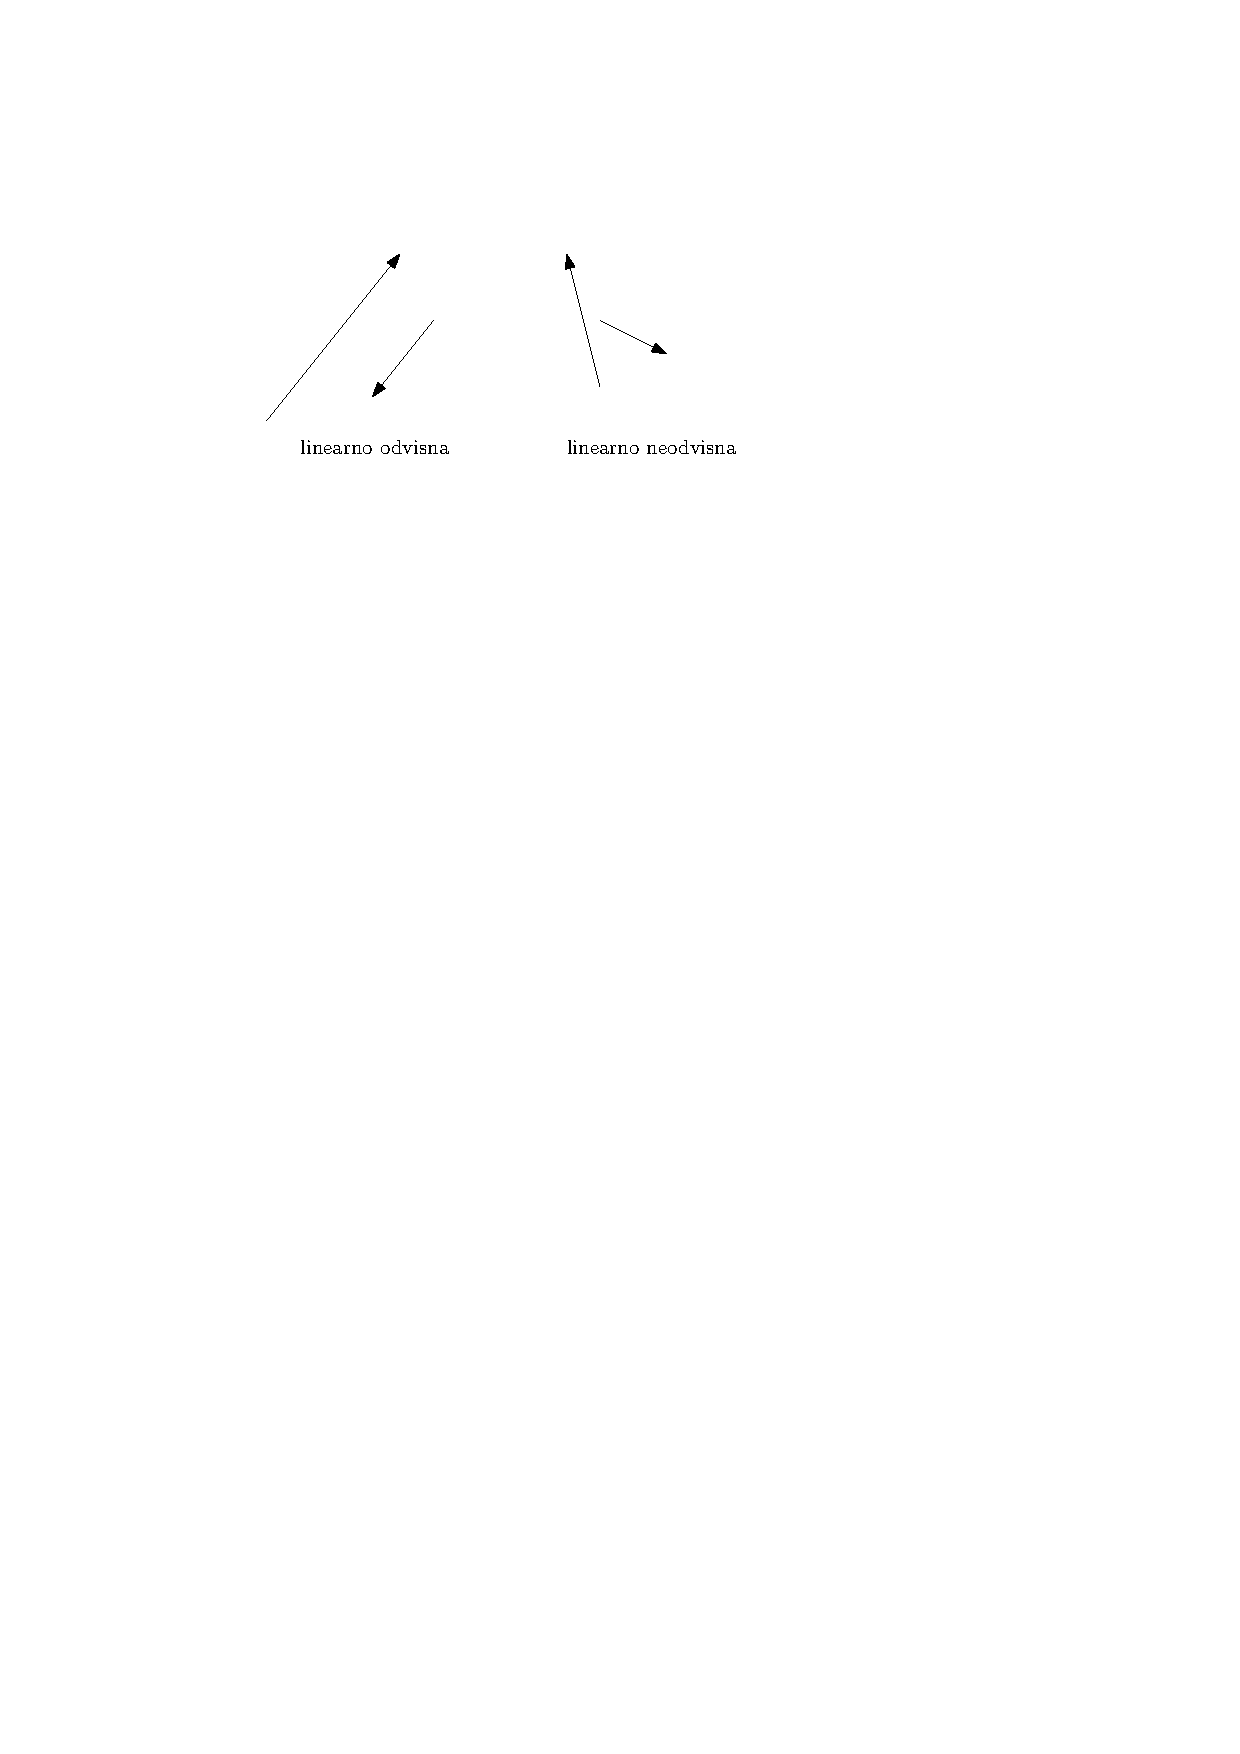
\includegraphics[width=0.5\textwidth]{odvisnost.pdf}
    \centering
\end{figure}

Vektorja $\vec{a}$ in $\vec{b}$ sta linearno neodvisna, če velja $m\vec{a}+n\vec{b}=0 \iff m=0=n$.

\section*{\textcolor{violet}{Utrjevanje}}
\textbf{\textcolor{violet}{Primere naredimo skupaj. Če dijaki dobro razumejo, lahko tudi individualno ali v tandemu.}}

\begin{zgled}
    V pravokotniku $ABCD$ sta bazna vektorja $\vec{a}=\vec{AB}$ in $\vec{b}=\vec{AD}$. Točka $T_1$ je razpolovišče $CD$, točka $T_2$ pa deli stranico $AB$ v razmerju $|AT_2|:|T_2 B|=1:2$. Izrazi vektorje $\vec{T_2 C}$, $\vec{T_1 B}$ in $\vec{T_2 T_1}$ v bazi. \textcolor{violet}{Nalogo rešimo skupaj s svetovanjem dijakov.}
\end{zgled}

\begin{zgled}
    Za bazna vektorja $\vec{a}$ in $\vec{b}$ določi $m,n\in\mathbb{R}$, če velja $(n-2)(\vec{a}+\vec{b})=3(m\vec{a}+\vec{b})$.
\end{zgled}

\begin{zgled}
    V pravilnem šestkotniku $ABCD$ z bazo $\vec{a}=\vec{AB}$ in $\vec{b}=\vec{AF}$ zapiši vektorje $\vec{BF}$ in $\vec{AD}$.
\end{zgled}

\begin{zgled}
    V pravokotniku $ABCD$ je točka $N$ razpolovišče stranice $BC$, točka $M$ pa leži na stranici $AB$ tako, da $|AM|:|MB|=3:2$. V kakšnem razmerju deli stranica $MD$ daljico $AN$. \textcolor{red}{Težja naloga: Na tablo nujno napišemo algoritem reševanja take naloge, ki naj ga dijaki prepišejo. Nalogo rešimo frontalno in smo posebej pozorni.}
\end{zgled}

\begin{zgled}
    V paralelogramu $ABCD$, je $E$ na stranici $CD$, da $|DE|:|DC|=1:5$, točka $F$ pa je presek $BE$ in $AC$. Pokaži, da velja $\vec{EF}=\frac{4}{9}\vec{EB}$. {Težja naloga enakega tipa: Rešujemo jo skupaj ob svetovanju dijakov.}
\end{zgled}

\begin{zgled}
    Pokaži, da težišče deli težiščnico v razmerju $2:1$. {Težja naloga podobnega tipa: Ko nalogo nastavimo, naj jo dijaki rešujejo individualno.}
\end{zgled}

\textbf{\textcolor{violet}{Dijaki si DN zabeležijo in odidejo iz razreda}}

\begin{example}
    Domača naloga 304, 311ac, 313, 314
\end{example}



\end{document}